\documentclass[10pt,a4paper]{article}

%%%%%%%%%%%%%%%%%%%%%%%%%%%
% MODIFY:

\newcommand{\authorA}{Jia Long Ji Qiu}
\newcommand{\authorB}{Jiabo Wang}
\newcommand{\authorC}{Yilun Liu}
\newcommand{\groupNumber}{J} % - YOUR GROUP NUMBER
\newcommand{\sourceCodeLink}{https://github.com/jialongjq/mlcms}

\newcommand{\workPerAuthor}{
\authorA&Task 1&1/4\\
      &Task 2&1/4\\
      &Task 3&1/4\\
      &Task 4&1/4\\
      &Task 5&1/4\\
      \hline
\authorB&Task 1&1/4\\
      &Task 2&1/4\\
      &Task 3&1/4\\
      &Task 4&1/4\\
      &Task 5&1/4\\
      \hline
\authorC&Task 1&1/2\\
      &Task 2&1/2\\
      &Task 3&1/2\\
      &Task 4&1/2\\
      &Task 5&1/2\\
}

%%%%%%%%%%%%%%%%%%%%%%%%%%%

%%
% imports for the exercise sheets
%

\usepackage[utf8]{inputenc}
\usepackage{amsmath}
\usepackage{amsfonts}
\usepackage{amssymb}

\usepackage[yyyymmdd]{datetime}
\renewcommand{\dateseparator}{--}

\usepackage[left=2cm,right=2cm,top=3cm,bottom=3cm]{geometry}
\usepackage{listings, xcolor}

\definecolor{codegreen}{rgb}{0,0.6,0}
\definecolor{codegray}{rgb}{0.5,0.5,0.5}
\definecolor{codepurple}{rgb}{0.58,0,0.82}
\definecolor{backcolour}{rgb}{0.95,0.95,0.92}

\lstdefinestyle{mystyle}{
    backgroundcolor=\color{backcolour},   
    commentstyle=\color{codegreen},
    keywordstyle=\color{magenta},
    numberstyle=\tiny\color{codegray},
    stringstyle=\color{codepurple},
    basicstyle=\ttfamily\footnotesize,
    breakatwhitespace=false,         
    breaklines=true,                 
    captionpos=b,                    
    keepspaces=true,               
    showspaces=false,                
    showstringspaces=false,
    showtabs=false,                  
    tabsize=2
}

\lstset{style=mystyle}

\usepackage{hyperref}

\usepackage{amsthm}
\newtheorem{lem}{Lemma}
\newtheorem{thm}{Theorem}
\newtheorem{cor}{Corollary}
\newtheorem{rem}{Remark}
\newtheorem{definition}{Definition}
\newtheorem{ter}{Terminology}

\usepackage{graphicx}

\newcommand{\M}{\mathcal{M}}
\newcommand{\N}{\mathcal{N}}
\newcommand{\K}{\mathcal{K}}
\newcommand{\SPDk}{\mathbb{P}^k}
\newcommand{\vol}{\text{vol}}

\newcommand{\Figref}[1]{Figure~\ref{#1}}
\newcommand{\figref}[1]{figure~\ref{#1}}
\newcommand{\Eqnref}[1]{Equation~(\eqref{#1})}
\newcommand{\eqnref}[1]{equation~(\eqref{#1})}

\usepackage{float}
\usepackage{tabularx}

\usepackage{fancyhdr}
\pagestyle{fancy}

\usepackage{totcount}
\newtotcounter{taskCounter}
\newtotcounter{pointCounter}
\newenvironment{task}[1]{\noindent\stepcounter{taskCounter}\textbf{Report on task #1}\smallbreak\hrule\smallbreak}{\smallbreak\hrule\bigbreak}

\usepackage{array}

\usepackage{caption}
\usepackage{subcaption}

\title{Report for exercise \exerciseNumber~from group~\groupNumber}

\makeatletter
\let\thetitle\@title
\let\theauthor\@author
\let\thedate\@date
\makeatother

\providecommand{\versiondate}{\today}

\lhead{Exercise sheet \exerciseNumber}
\chead{Master Praktikum: Modelling and Simulation of Crowds WS2022/23}
\rhead{TUM}
\lfoot{Report of Group \groupNumber}
\cfoot{\thepage}
\rfoot{Last compiled: \versiondate}
\renewcommand{\headrulewidth}{0.4pt}
\renewcommand{\footrulewidth}{0.4pt}

\newcommand{\frontpage}{
\begin{center}
\textbf{\thetitle}\\~\\
\end{center}
\begin{table}[H]
\begin{tabular}{ll}
Tasks addressed:&\total{taskCounter}\\
Authors:&\authorA\\
&\authorB\\
&\authorC\\
Last compiled:&\versiondate\\
Source code:&\sourceCodeLink
\end{tabular}
\end{table}
\vfill
The work on tasks was divided in the following way:
\begin{table}[H]
\begin{tabularx}{\textwidth}{X|p{2cm}|p{2cm}}
\workPerAuthor
\end{tabularx}
\end{table}
\newpage
}

\begin{document}

\frontpage

\bigskip
\begin{abstract}
\bigskip
In crowd modelling one important thing is the ability to represent pedestrian behaviours and dynamics as realistic as possible. However, this is not a trivial task since such dynamics tend to occur in complex circumstances, either because there are many interactions within the crowd itself or because of the complexity in the geometry of an scenario.

In this project we are going to focus on the speed of pedestrians and how can this behaviour be predicted. There are many computational models, also called classical models, that are generally decision-based, velocity-based or force-based approaches. In those models, a certain behaviour can be adjusted with some given inputs, which have physical interpretations. However, the problem with these models is that accurate predictions are difficult to achieve given complex circumstances.

Another way of making these behaviour predictions consists in the use of artificial neural networks. Artificial neural networks are data-based models, which means that it makes these predictions based on previous observations. Since neural networks can have a lot of parameters, they are able to reproduce complex patterns.

So now the question is, can a neural network model make more accurate predictions than a classical model? This is, in fact, what we want to prove empirically through this project.
\end{abstract}

\newpage

\begin{task}{1, Description of models and data sets}

The pedestrian modelling approaches are continuous speed models based on the $K = 10$ closest neighbours. We denote in the following $(x, y)$ as the position of the considered agent, $v$ as its speed and $((x_i,y_i),i = 1,...,K)$ as the positions of the K closest neighbours.

The Weidmann model is a fundamental diagram based model, which means that there's a relation between speed and local density. It describes the speed $v$ as the product of a desired speed $v_0$ with a term that scales it depending on several factors, which are the mean spacing $\bar{s}_{K}$, the desired speed itself, the time gap $T$ and the pedestrian size $l$.

\begin{equation} 
    v = FD(\bar{s}_{K}, v_0, T, l) = v_0(1-e^{\frac{l-\bar{s}_{K}}{v_{0}T}})
    \label{weidmann}
\end{equation}

\begin{equation}
    \bar{s}_{K} = \frac{1}{K} \sum_{i = 1}^{K} \sqrt{(x - x_{i})^{2} + (y - y_{i})^{2}}
    \label{mean_space}
\end{equation}

The second modelling approach is a feed-forward Artificial Neural Network (ANN) with hidden layers H.
\begin{equation}
    v = NN(H, \bar{s}_{K}, (x_{i} - x, y_{i} - y, 1 \leq i \leq K))
\end{equation}

The Neural Network has $2K + 1$ inputs, which are the K relative positions and the mean spacing $\bar{s}_{K}$. And the number of parameters in the network depends on the number of nodes in the hidden layers.

\bigskip

As this final project is based on Tordeux's paper \cite{Tordeux}, we are going to use the same data sets for comparing the FD-based and ANN modelling approaches, and try to recreate their results. There are two data sets that are available on the internet \cite{DataSet}, which are part of the online database of pedestrian experiments.

The first dataset is called the ring experiment and comes from a experiment done on a closed geometry of length 30 m and width 1.8 m for different density levels (ranging from 0.25 to 2 ped/m2 — the participant number ranges from 15 to 230).

\begin{figure} [H]
    \centering
    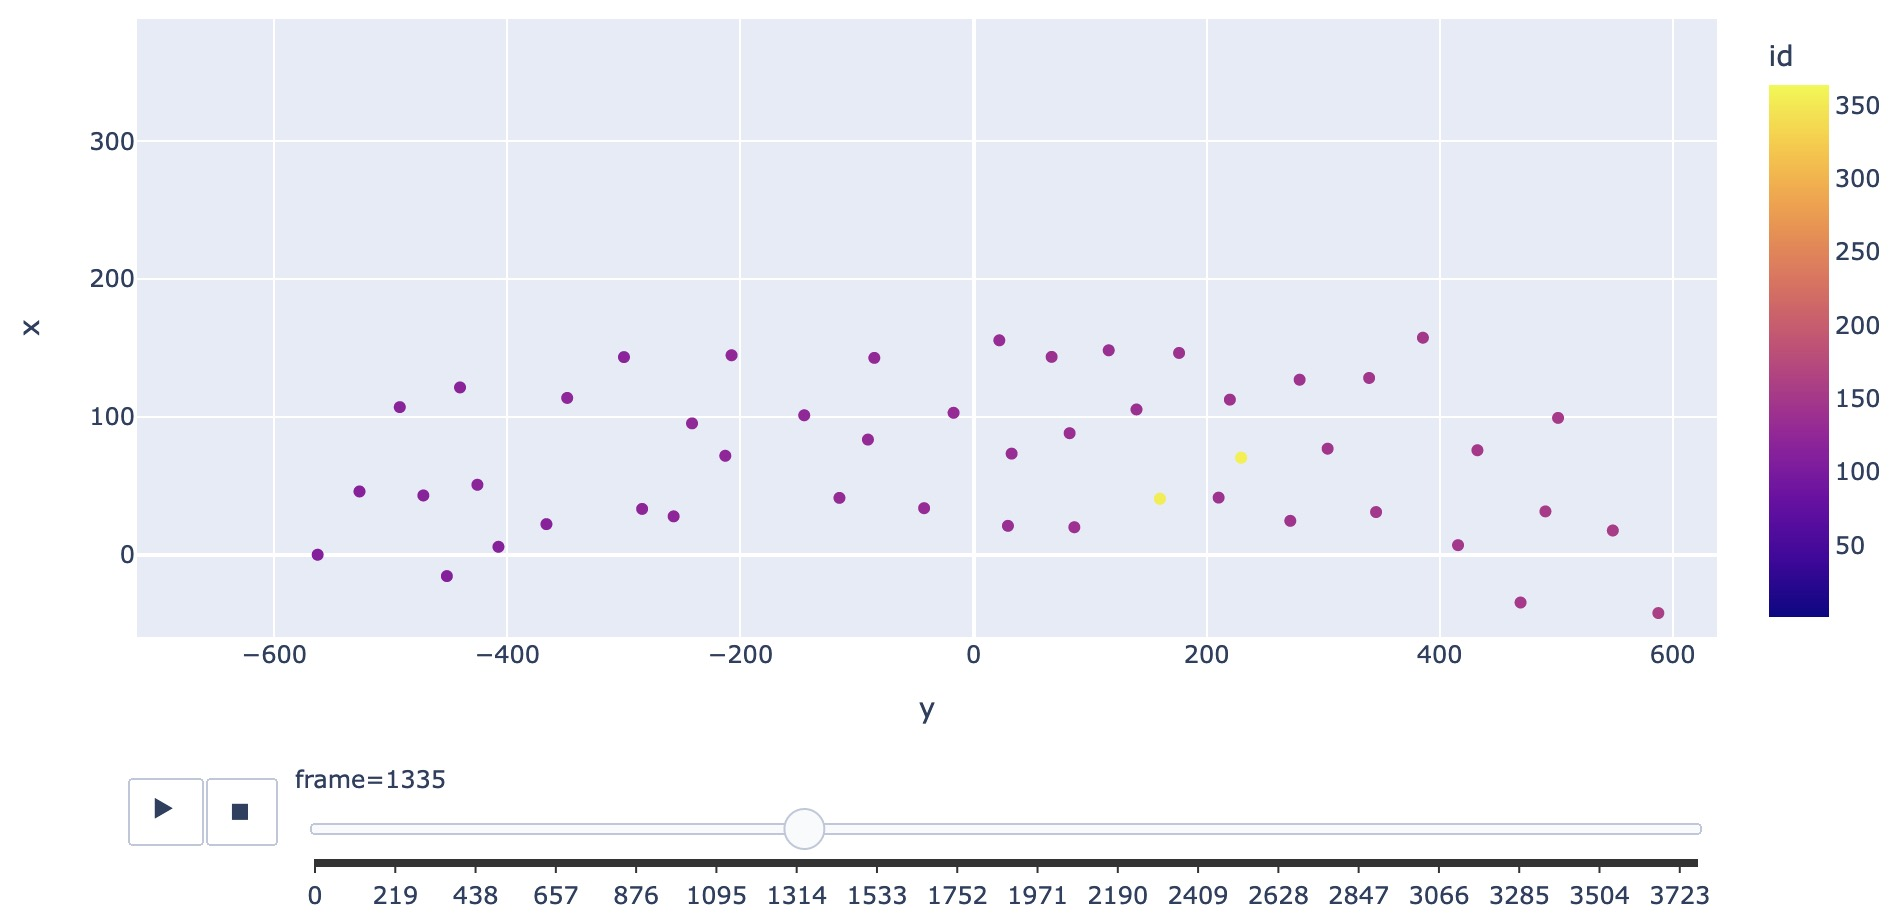
\includegraphics[width=15cm]{images/corridor.jpg}
    \caption{Trajectory of the pedestrians in the ring experiment}
    \label{corridor}
\end{figure}

\newpage

The second dataset is an experiment for a bottleneck geometry. The width of the system in front of the bottleneck is 1.8 m while the width of the bottleneck varies (from 0.70, 0.95, 1.20 to 1.80 m — 150 participants by experiment).

\begin{figure} [H]
    \centering
    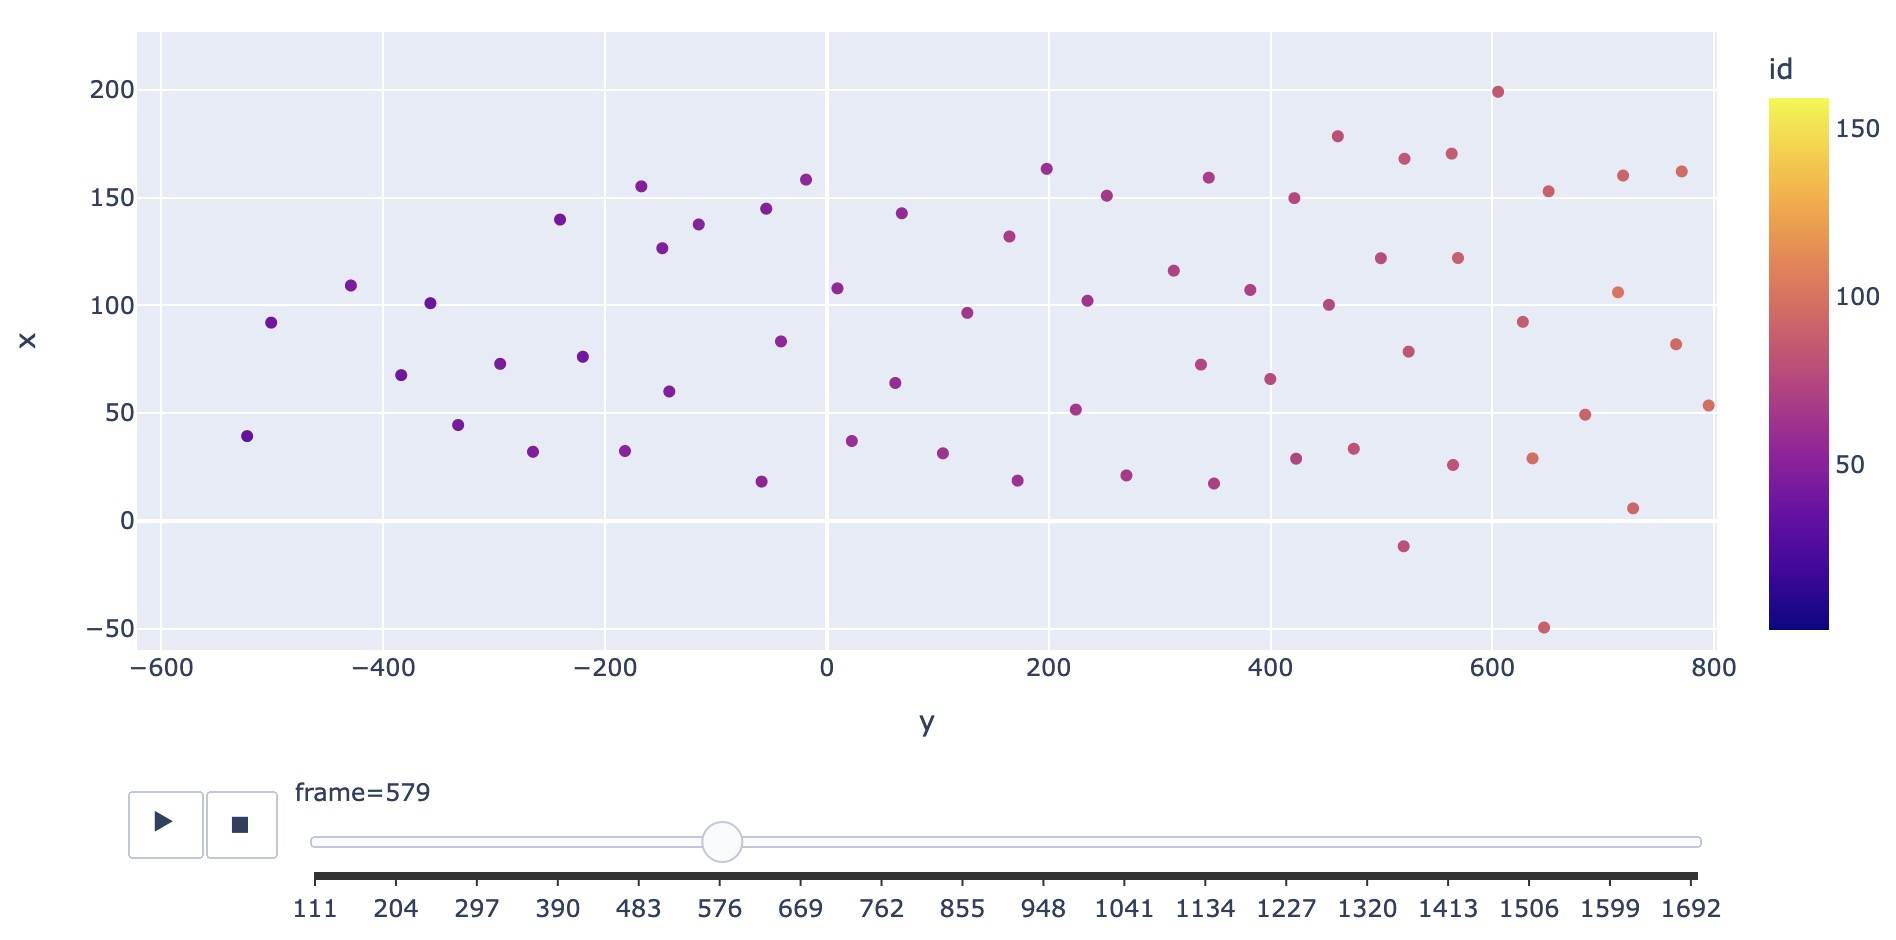
\includegraphics[width=15cm]{images/bottleneck.jpg}
    \caption{Trajectory of the pedestrians in the bottleneck experiment}
    \label{bottleneck}
\end{figure}

\end{task}

\newpage

\begin{task}{2, Data preprocessing and implementation of the models}

\subsubsection*{Part 1: Data preparation}

Before implementing the main part of our project, we have to prepare the data in order to fit both the Weidmann model and the neural network model. The data preprocessing has been done as follows:
\begin{enumerate}
    \item Calculate the distance matrix of all present pedestrians for each time frame;
    \item Create records of each pedestrian's distances to the 10 nearest neighbors for each time frame (as input for the NN model)
    \item Calculate the mean spacing defined in \eqref{mean_space} (as input for both the NN model and the Weidmann model);
    \item Create records of each pedestrian’s velocity by calculating difference between adjacent time frames (as test output for both model).
\end{enumerate}

The data preparation corresponds to the function \texttt{generate\_dataset()} in the file \texttt{utils.py}:
\begin{lstlisting}[language=Python]
def generate_dataset(dfs, K):
    '''
    Generate desired dataset for dataframes collected in a scenario.
    In the original dataframe are the records of coordinates '(x, y, z)' for each pedestrians on different time frames, 
    from which records of distances to k-nearest-neighburs (X) and velocity (y) could be calculated.

    :param dfs: a list of dataframes collected within a certain scenario
    :param K: number of nearest neighbors to keep in the dataset
    :returns: a tuple of X (input) and y (output) for the dataset
    '''
    dataset_X = []
    dataset_y = []

    # for each given dataframe in the scenario
    for data in dfs:
        # generate dictionaries of id, coordinates and distance matrix on each time frame 
        id_frame_dict = {}
        coords_frame_dict = {}
        dist_frame_dict = {}
        for frame in range(min(data['frame']), max(data['frame'])+1):
            tmp = data[data['frame']==frame]
            ids = list(tmp['id'])
            coords = list(tmp['coords'])
            
            id_frame_dict[frame] = ids
            coords_frame_dict[frame] = dict(zip(ids, coords))
            dist_frame_dict[frame] = dict(zip(ids, distance.cdist(coords, coords, 'euclidean')))
        
        # generate dictionaries of the list of distance to neighbors and velocity across time frames on each id
        dist_list_id_dict = {}
        velocity_list_id_dict = {}
        for id in range(min(data['id']), max(data['id'])+1):
            tmp = data[data['id']==id]
            dist_list = []
            velocity_list = []
            for frame in range(min(tmp['frame']), max(tmp['frame'])):
                dist_list.append(sorted(dist_frame_dict[frame][id]))
                velocity_list.append(np.linalg.norm(np.subtract(coords_frame_dict[frame][id], coords_frame_dict[frame+1][id])))
            dist_list_id_dict[id] = dist_list
            velocity_list_id_dict[id] = velocity_list

        # generate record lists of X (distance to neighbors) and y (velocity) as the model's input and output
        data_X = []
        data_y = []
        for id in range(min(data['id']), max(data['id'])+1):
            data_X += dist_list_id_dict[id]
            data_y += velocity_list_id_dict[id]

        # select and prune the records into distances to K nearest neighbors
        for X, y in list(zip(data_X, data_y)):
            if len(X) > K:
                dataset_X.append([i / 10 for i in X[1:K]])
                dataset_y.append(y / 10)

    return (dataset_X, dataset_y)
\end{lstlisting}


\subsubsection*{Part 2: Weidmann model}

Having the data prepared for the Weidmann model, all we had to do was to compute the predicted speed by applying the formula \eqref{weidmann}. As for measuring the error and see how well the model is fitting the data, we have selected three different metrics, which are the mean absolute error (MAE), the mean squared error (MSE) and the ${R^2}$ score.


\begin{lstlisting}[language=Python]
def weidmann_model(x, v0, l, T):
    '''
    Weidmann Model Function
    :param x: mean distance to k nearest neighbors
    :param v0: desired speed
    :param l: pedestrian size
    :param T: time gap
    '''
    return v0 * (1 - np.exp((l - x) / v0 / T))
\end{lstlisting}

It is worth noting that we fitted the parameters in the Weidmann model by ourselves instead of directly using the ones given in the paper, as they cannot give correct results. The fitting of this non-linear function was carried out by using \texttt{curve\_fit} from \texttt{scipy\.optimize}:

\begin{lstlisting}[language=Python]
bottleneck_popt, bottleneck_pcov = curve_fit(weidmann_model, bottleneck_X_mean_train, bottleneck_y_train)

corridor_popt, corridor_pcov = curve_fit(weidmann_model, corridor_X_mean_train, corridor_y_train)

bottleneck_corridor_popt, bottleneck_corridor_pcov = curve_fit(weidmann_model, bottleneck_corridor_X_mean_train, bottleneck_corridor_y_train)
\end{lstlisting}

\subsubsection*{Part 3: Artificial neural network model}

For the artificial neural network approach, we build a function to accept input of different structures as nodes in each hidden layer, along with traning set, and returning a trained model.


\begin{lstlisting}[language=Python]
def NN(layers, X_train, y_train, n_splits=5, epochs=20):
    '''
    Implement and train a Neural Network with the assigned structure.
    :param layers: number of nodes on each hidden layer, representing the structure of the Neural Network
    :param X_train, y_train: training set input and output
    :param n_splits: K-fold validation parameter
    :param epochs: number of epochs in total during the training process
    '''
    model = Sequential()
    
    model.add(Dense(layers[0], input_shape=(X_train.shape[1],), activation='relu'))
    if len(layers)>=2:
        for i in layers[1:]:
            model.add(Dense(i, activation='relu'))
    model.add(Dense(1))

    model.compile(optimizer='adam', loss='mean_squared_error')
    
    kfold = KFold(n_splits=n_splits, shuffle=True, random_state=1)
    scores = []
    count = 0
    for train_index, val_index in kfold.split(X_train):
        count += 1
        print("Training Process:", count, '/', n_splits, "Fold")
        X_train_bootstrap, X_val_bootstrap = X_train[train_index], X_train[val_index]
        y_train_bootstrap, y_val_bootstrap = y_train[train_index], y_train[val_index]
        
        X_train_boostrap_resampled, y_train_bootstrap_resampled = resample(X_train_bootstrap, y_train_bootstrap)
        model.fit(X_train_boostrap_resampled, y_train_bootstrap_resampled, epochs=int(epochs/n_splits), batch_size=32, verbose=2)
        score = model.evaluate(X_val_bootstrap, y_val_bootstrap, verbose=0)
        scores.append(score)
        
    print("\nK-Fold Validation MSE: %.2f" % np.mean(scores))
    return model
\end{lstlisting}

The neural network uses ReLU as activation function, with Adam optimizer and MSE as loss function. The neural network is fitted with 5-fold cross-validation and bootstrap. The training process was carried out with 20 epochs in total and a batch size of 32 for each structure of NN. 
\end{task}
\newpage

\begin{task}{3, Test of different NN structure on Bottleneck scenario}
In this part we would like to test the performance of NN with different structures and select the one with best result for further testing. Without loss of generality, we implement our experiment on the Bottleneck scenario.

After finishing training and testing our neural networks with structures of 1, 2, 3, 4+2, 5+2, 5+3, 6+3 and 10+4 nodes in the hidden layer, from which we could evaluate their MSE measure on both the training set (validation error) and the test set. The result of different structures along with Weidmann Model is shown in figure \ref{MSE-b}.

\begin{figure} [H]
    \centering
    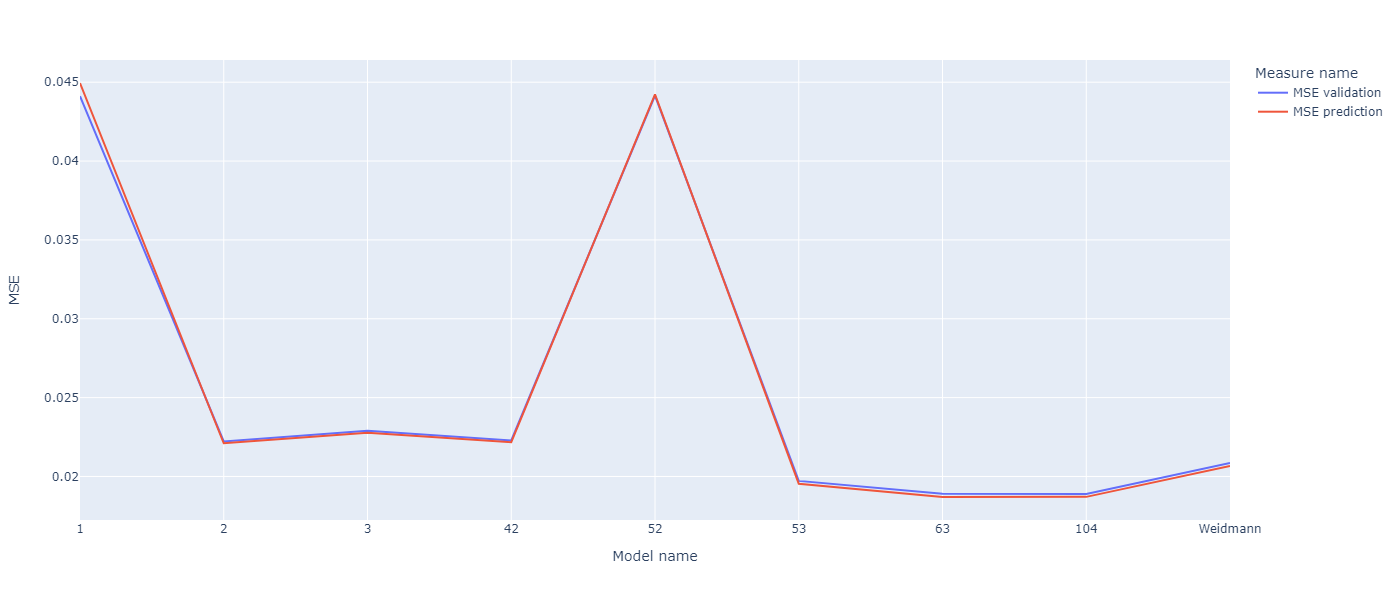
\includegraphics[width=17cm]{images/MSE of different structures for Bottleneck.png}
    \caption{MSE for different structure of NN on the Bottleneck dataset}
    \label{MSE-b}
\end{figure}

Surprisingly, our model yields results that are different from those mentioned in the paper. As we chose a smaller number of epochs and validation folds (20 epochs in total, 5-fold validation, enough to guarantee a convergence of loss in the experiment) comparing to the original process they performed (50 subsamples, no other detail given), our model did not over-fit the data very badly, as we can see in the plot that the validation error is similar to the prediction error. 

More over, the structure with best performance in our experiment turned out not to be the one with 3 nodes as in the paper, but the one with 6+3 nodes and 2 hidden layers. This might because the difference in choice of loss function and optimizer, as no further related information were given in the paper. And We can still observe a canonical behaviour of NN that the training error tends to decrease as we increase the complexity of the network, while the testing error shows a minimum before rising again (overfitting at 10+4 nodes).

\end{task}

\newpage

\begin{task}{4, Model Comparison}
To compare the result from Weidmann model and NN model more thoroughly, we first test Weidmann model's prediction in the bottleneck and corridor scenario with parameters fitted on different cases.


\begin{figure} [H]
    \centering
    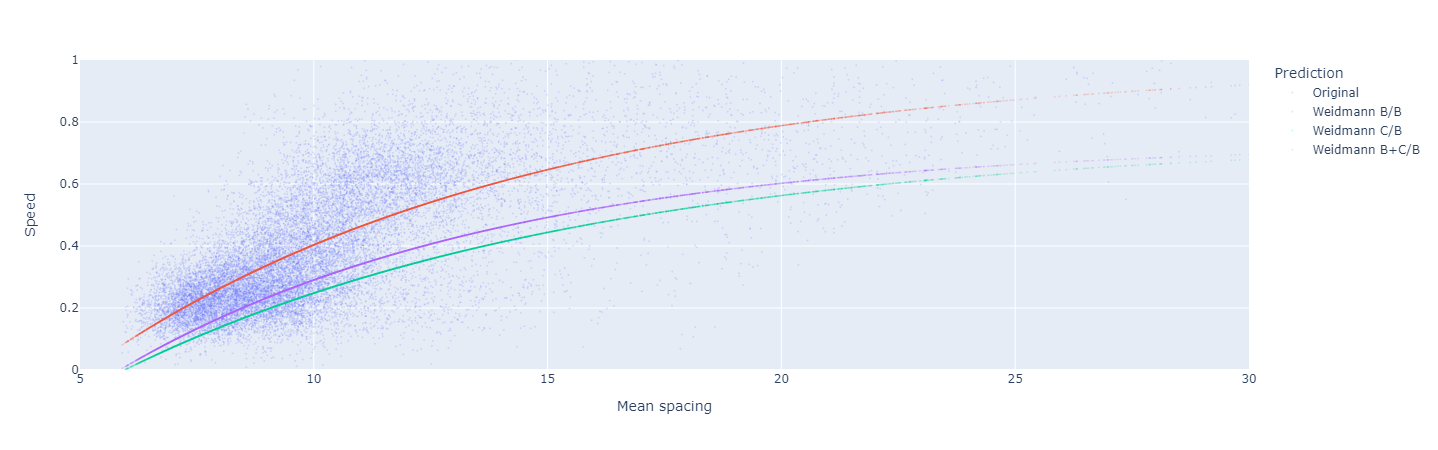
\includegraphics[width=15cm]{images/Weidmann-b.png}
    \caption{Weidmann model's prediction on Bottleneck scenario, with parameters fitted on Bottleneck, Corridor and both 2 scenarios}
    \label{Weidmann-b}
\end{figure}

\begin{figure} [H]
    \centering
    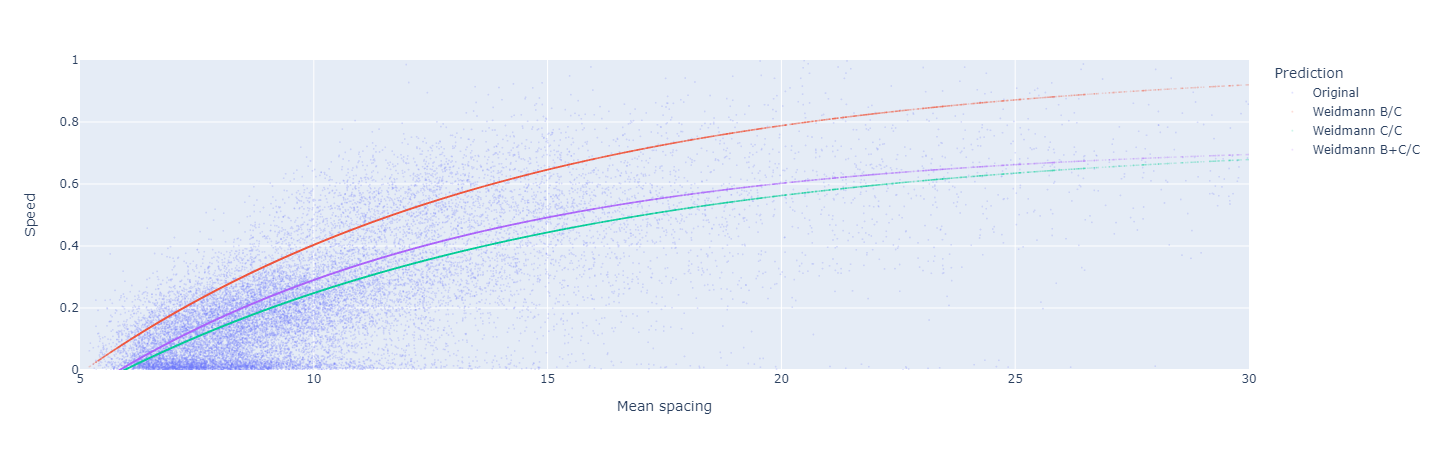
\includegraphics[width=15cm]{images/Weidmann-c.png}
    \caption{Weidmann model's prediction on Corridor scenario, with parameters fitted on Bottleneck, Corridor and both 2 scenarios}
    \label{Weidmann-b}
\end{figure}

Afterwhich we test the result of using NN with 3 (best structure on paper) and 6+3 (best structure from task 3) nodes and compare them to results from Weidmann model respectively.

\begin{figure} [H]
    \centering
    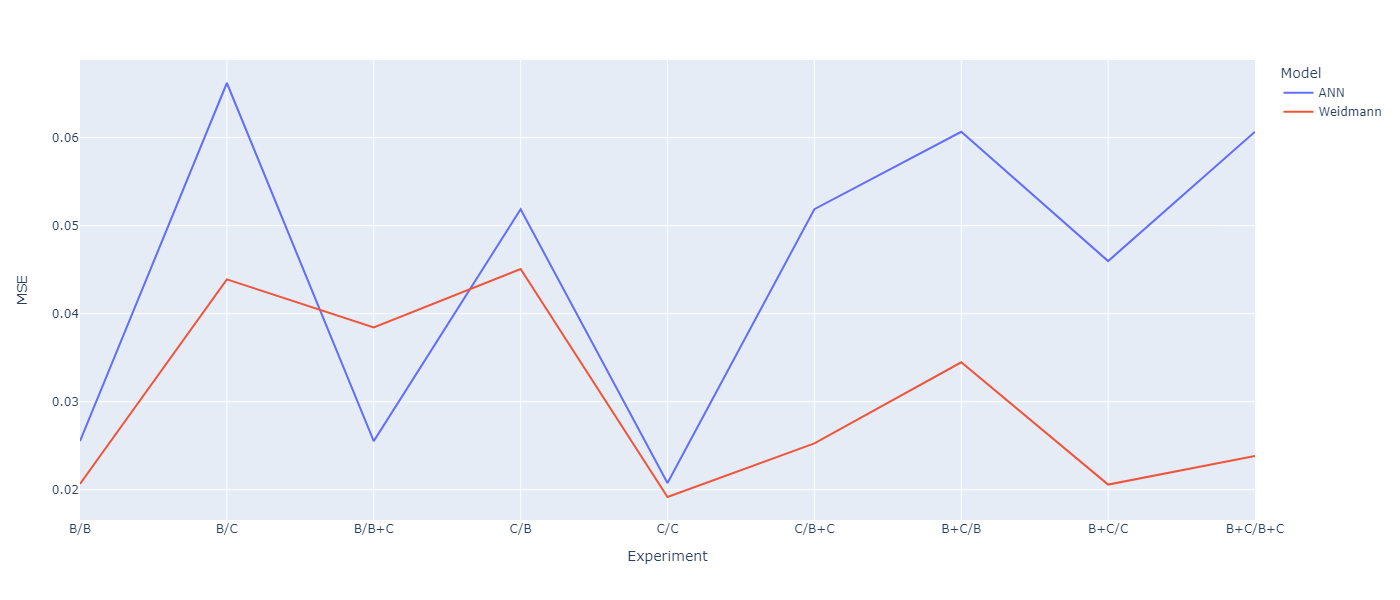
\includegraphics[width=15cm]{images/Compare_3.png}
    \caption{Comparing MSE performance of Weidmann model and NN with 3 nodes, trained and tested on different combinations of Bottleneck, Corridor and both scenarios}
    \label{Weidmann-b}
\end{figure}


\begin{figure} [H]
    \centering
    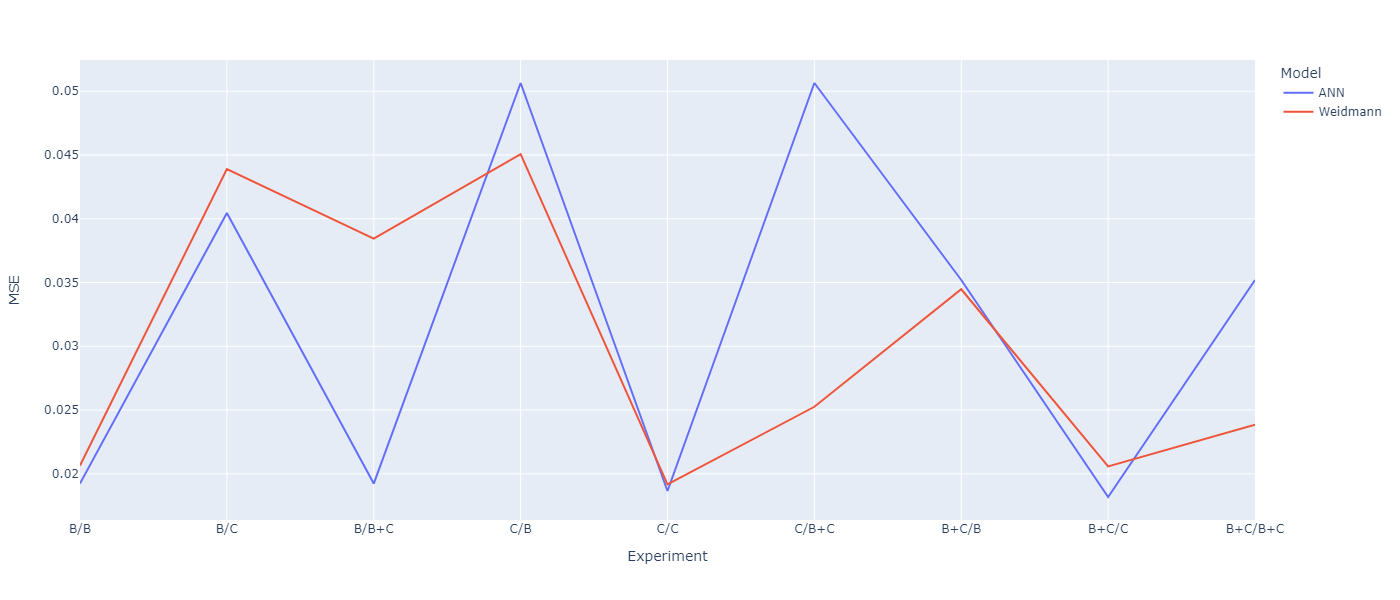
\includegraphics[width=15cm]{images/Compare_6+3.png}
    \caption{Comparing MSE performance of Weidmann model and NN with 6+3 nodes, trained and tested on different combinations of Bottleneck, Corridor and both scenarios}
    \label{Weidmann-b}
\end{figure}

As we expect that the NN model with 3 nodes does not give good results, whereas 6+3 structure has achieved a lower MSE on many of the experiments.

\begin{table}[H]
    \centering
    \caption{MSE performace ratio of NN (6+3) to Weidmann Model}
    \begin{tabular}{c|c}
        Experiment & MSE ratio \\
        \hline
        B/B & 0.9312 \\
        B/C & 0.9214 \\
        B/B+C & 0.5004 \\
        C/B & 1.1236 \\
        C/C & 0.9730 \\
        C/B+C & 2.0050 \\
        B+C/B & 1.0211 \\
        B+C/C & 0.8834 \\
        B+C/B+C & 1.4760
    \end{tabular}
    \label{tab}
\end{table}

Comparing to Weidmann Model, the NN model with 6+3 nodes achieved a 50\% reduction of MSE in the experiment of using Bottleneck scenario as training set and 2 scenarios together as test set. 

\end{task}

\newpage

\begin{task}{5, Discussion of the approach and architecture}
Besides the discussion of MSE measure in Task 4, we would also like to look into the distribution of prediction of the two models:

\begin{figure} [H]
    \centering
    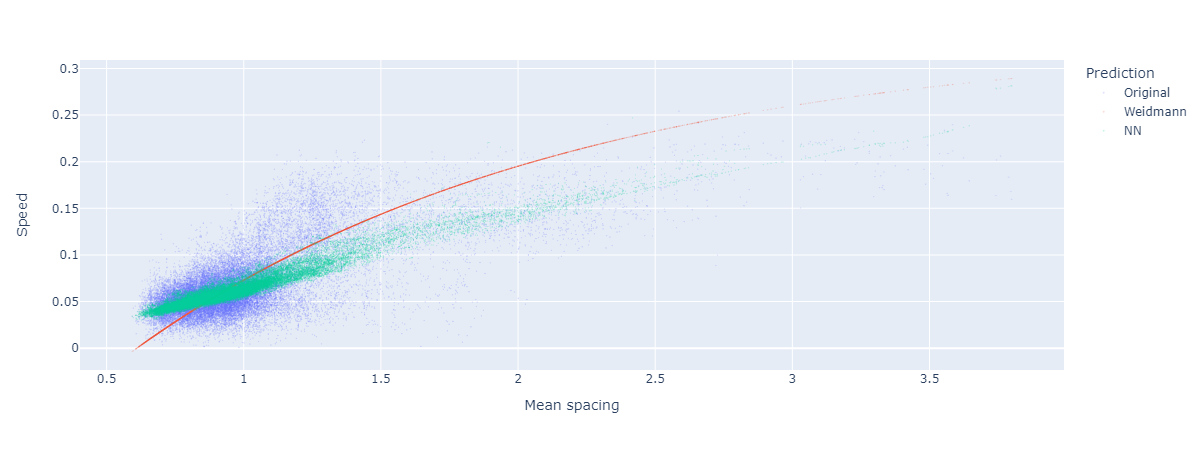
\includegraphics[width=15cm]{images/Comparing NN-3 and Weidmann on test set.png}
    \caption{Comparing distribution of prediction given by NN (6+3) and Weidmann on Bottleneck scenario}
    \label{compare}
\end{figure}

We can see that the results given by Weidmann model is a line as it is simply a non-linear function of the speed to mean spacing, whereas the NN has a wider distribution as it not only considered the mean spacing, but all the distances to nearest neighbors. This gives it a chance to fit the real data distribution better by capturing potential impart factors which Weidmann model fails to take into consideration. Such powerful ability was guaranteed by neural network's characteristics so as to consider higher dimensional features and model these complex non-linear relationships hidden behind the data distribution, compared to a simple non-linear model.

\end{task}


\newpage
\bibliographystyle{plain}
\bibliography{Literature}
\begin{thebibliography}{9}

\bibitem{Tordeux}
Tordeux, A., Chraibi, M., Seyfried, A., and Schadschneider, A. (2019).
Prediction of pedestrian dynamics in complex architectures with artificial neural networks.
Intelligent Transportation Systems, 24(6):556–568.

\bibitem{DataSet}
Tordeux, A., Chraibi, M., Seyfried, A., Schadschneider, A.: Data from: Prediction of Pedestrian Speed with Artificial Neural Networks (2017). DOI 10.5281/zenodo.1054017. URL \url{https://doi.org/10.5281/zenodo.1054017}
\end{thebibliography}

\end{document}